\section{Experiments}
\label{sec:experiments}
I applied above techniques on real world dynamic data.
This section would reveal more implementation details and parameter settings, and also provide results and observations from experiments.

\subsection{Landmark detection results}
\label{sec:landmark_detection_results}
First I conducted a prior experiment before further developing landmark detection techniques by answering the question: How would landmark dynamics affect final airway analysis?

I studied this on the first dynamic data I got from a doctor.
This 59 days subject only had a dummy TVC \footnote{TVC was not visible due to the doctor's choice of scan area. I then chose the top of the airway as a dummy landmark TVC} and TC for registration.
I manually annotated the these two landmarks in each frame and computed the Euclidean difference between landmarks with respect to time.

Figure~\ref{fig:landmark_dynamics} showed the landmark dynamics between each frame in millimeter.
In this figure, TC had a significant changes after time step 4.
The landmark dynamics revealed that airway of the subject was changing a lot in a period of time.
This observation matched our measurement of cross-sectional areas.

Figure~\ref{fig:landmark_updated} showed the results of airway measurement of the 59 days subject.
The different between two is whether considering the landmark dynamics.
One neglected landmark dynamics and the other used updated landmarks in each time steps.
We can see that Figure~\ref{fig:landmark_updated} (right) captured a cross-sectional area drop around depth 0.8.
Figure~\ref{fig:landmark_updated} (left), however, lost this feature (aware difference between the green curves on the left and on the right.)
Because an area drop is a critical feature for airway analysis, I considered updating landmarks in each time frame is an important issue and further developed the framework described in Section~\ref{sec:landmark_detection}.

\begin{figure}[tb]
  \begin{center}
    \begin{tabular}{ccc}
    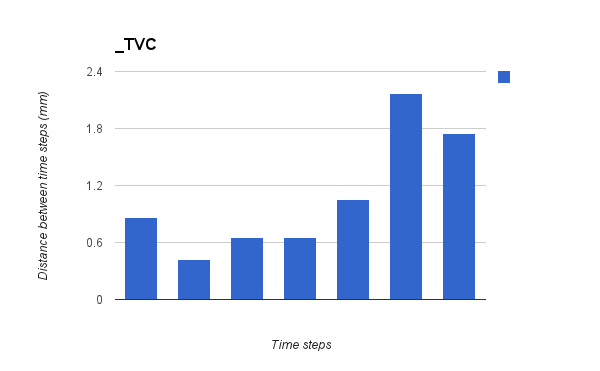
\includegraphics[height=35mm] {fig/d_TVC.png}
    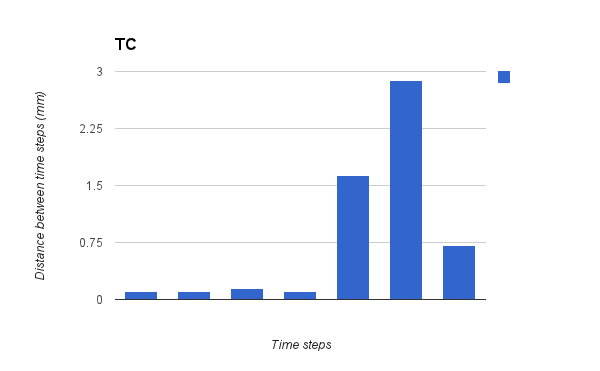
\includegraphics[height=35mm] {fig/dTC.png}
    \end{tabular}
    \caption{ \label{fig:landmark_dynamics} Visualization of the landmark dynamics of a 59 days subject. 
    }
  \end{center}
\end{figure}

\begin{figure}[tb]
  \begin{center}
    \begin{tabular}{ccc}
    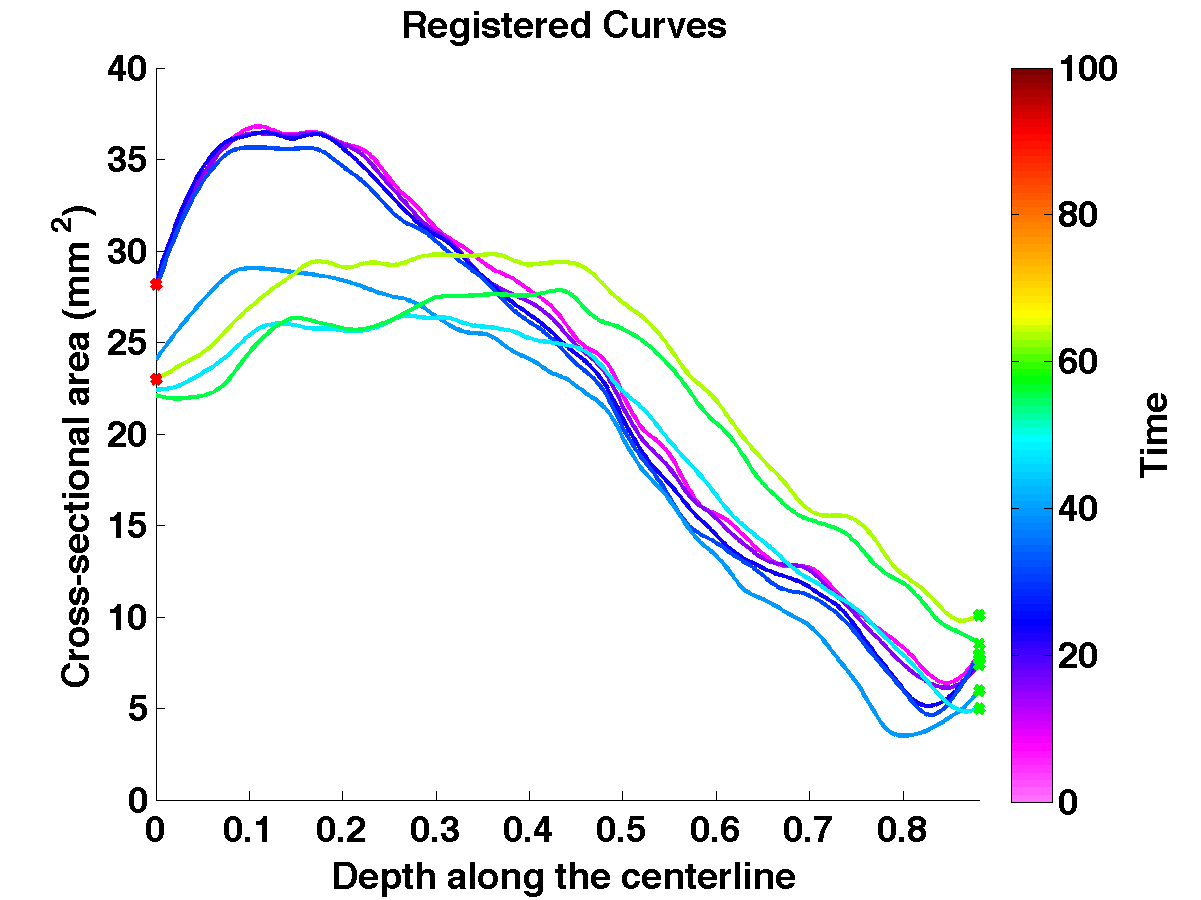
\includegraphics[height=35mm] {fig/registered_1_updates_0.png}
    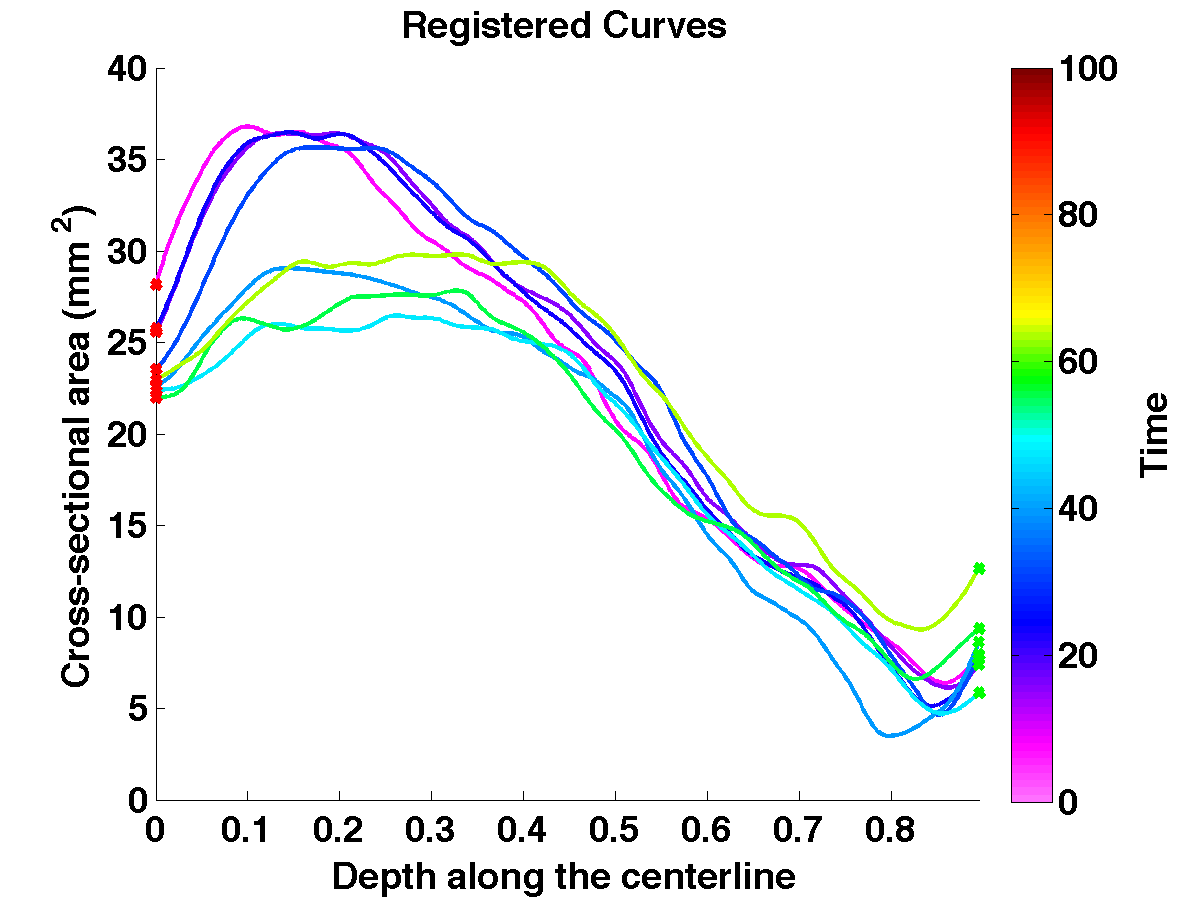
\includegraphics[height=35mm] {fig/registered_1_updates_1.png}
    \end{tabular}
    \caption{ \label{fig:landmark_updated} Cross-sectional area of a 59 days subject with different registration landmarks. The left figure showed the result with same landmarks for each time steps. The right figure showed the results with updated landmarks for each time steps. Note that in depth around 0.8, a lower cross-sectional measurement was disappear in the left but remained in the right.
    }
  \end{center}
\end{figure}

{\bf Training.} 
The training set had 95 3D CT images with manually annotated landmarks from nasal spine, choana, epiglottis tip, TVC, and TC.
I trained a linear SVM classifier for TC using concatenating HOG features.
Each subject provided a positive example which would be HOG features extracting from three orthogonal bounding boxes passed through the landmark TC.
The scale of the bounding boxes was determined by twice of the minimum rectangle covered the airway in the axial plane.
The negative examples were drawn in random scale and location that not intersected with the positive bounding boxes.

{\bf Detection.}
In our case, I utilized a prior of geometry to eliminate possible hypotheses.
In each depth I only drew one hypothesis from the center of the airway using the scale with the same heuristic in training.
The trained SVM classifier predicted a score of the landmark likelihood given different depth.
Figure~\ref{fig:landmark_detection} illustrated the likelihood prediction on training data.
We can see there are some outliers in prediction on the training data.
Due to these outliers, the mean prediction error was 24.7436 (mm) and the standard divination was 29.4251 (mm).

\begin{figure}[tb]
  \begin{center}
    \begin{tabular}{ccc}
    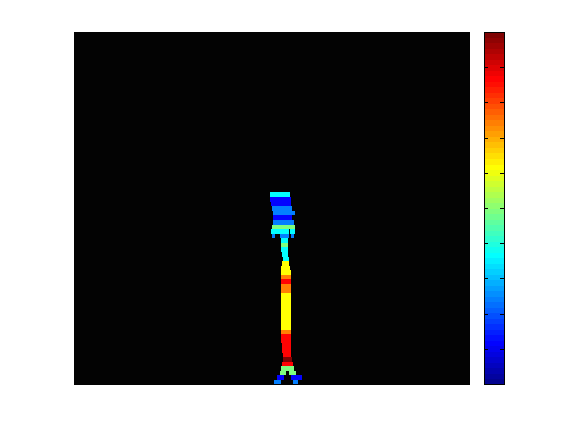
\includegraphics[height=35mm] {fig/CRL02_TracheaCarina_left.png}
    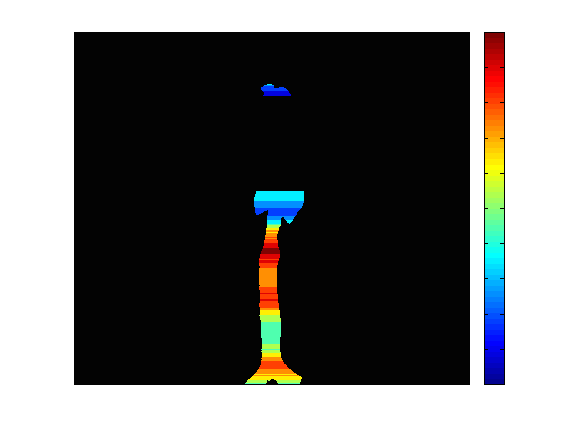
\includegraphics[height=35mm] {fig/CRL04_TracheaCarina_left.png}
    \end{tabular}
    \caption{ \label{fig:landmark_detection} Illustration of the likelihood of landmark TC. In most of case the detector can locate TC in a correct position (left). Even some fail cases still nominated the correct TC position as their second or third choice (right).
    }
  \end{center}
\end{figure}

Now let us try to apply the detector on dynamic data and see if it can handle landmark dynamics against the system dynamics.
I applied the detector on a 134 month subject (Fleck-005).
Table~\ref{tab:landmarks} summarized the errors of landmark prediction on TC for which neglecting landmark dynamics, and my landmark detector using concatenating HOG (HOG3)\footnote{One outlier is removed. Count the outlier than the mean would be 3.9280 mm (12.7448 px) and the std. would be 4.4680 mm (15.0649 px).}.
My automatically landmark detector reduced the errors of the mean and standard deviation.
However, the problem of outliers reminded in one time frame.
The current landmark detection framework did a decent job yet there are some spaces of improvement.

\begin{table}
  \centering
   \caption{Errors of landmark prediction methods of a 134 month subject (Fleck-005).
   }
  \begin{tabular}{rcccc}
  & mean (mm) & std. (mm) & mean (px) & std. (px) \\
  \hline
  None & 4.7575 & 2.5314 & 18.6614 & 10.2052 \\
  HOG3 & 2.8812 & 1.6134 & 9.3357 & 6.6279 \\
  \end{tabular}
  \label{tab:landmarks}
\end{table}

\begin{figure}[tb]
  \begin{center}
    \begin{tabular}{ccc}
    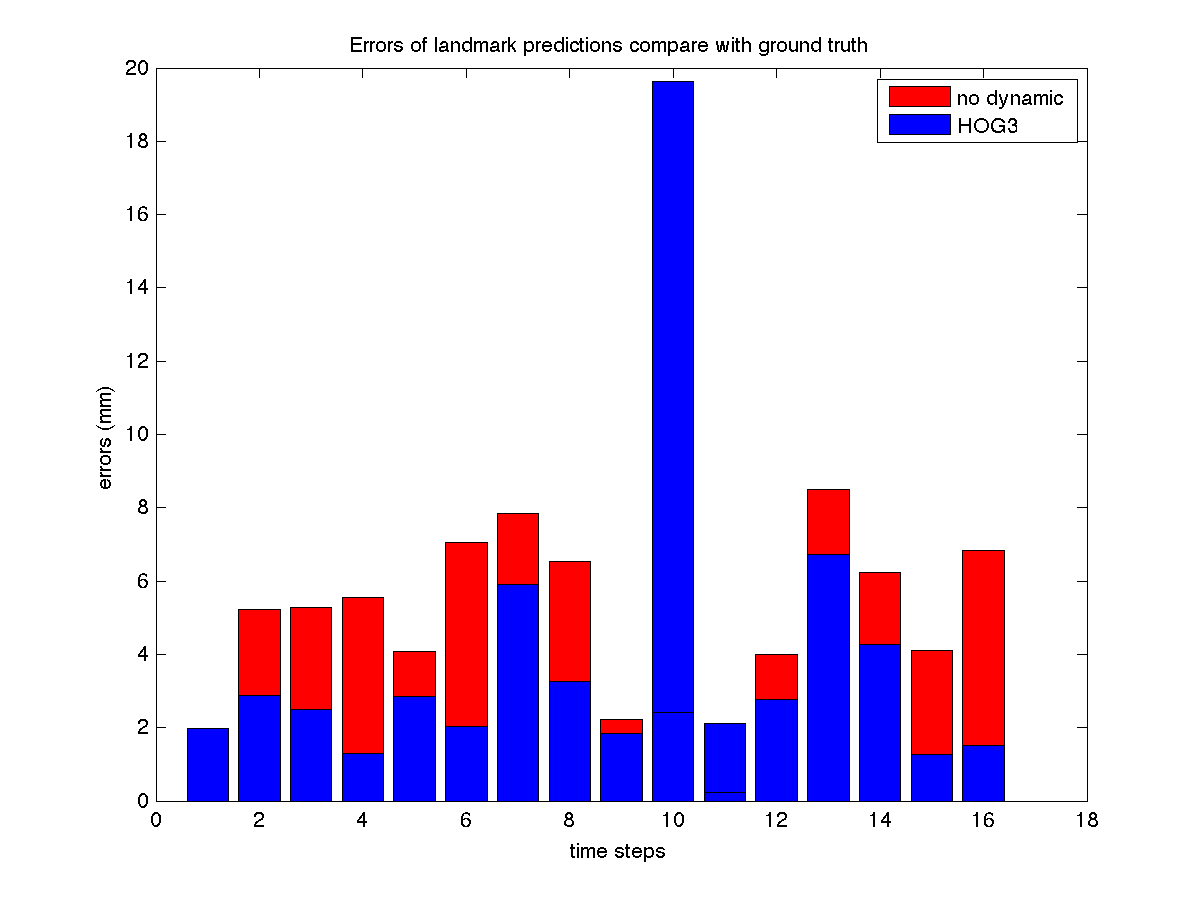
\includegraphics[height=35mm] {fig/landmark_errors.png}
    \end{tabular}
    \caption{ \label{fig:landmark_errors} Illustration of the landmark prediction errors in each time step. Red bar showed the errors of neglecting landmark dynamics and blue bar showed the errors from algorithm. Note that there is an outlier in time step 10.
    }
  \end{center}
\end{figure}

\subsection{Dynamic airway analysis}
\label{sec:dynamic_airway_analysis}
I performed dynamic airway analysis using functional boxplots on real world data given by a physician.
The normal control atlas was built from 68 health subjects in control group used the method in~\cite{hong2014statistical}.
Figure~\ref{fig:Fleck} showed the results.
Here I compared these results with the comments from the doctor of two cases.

{\bf Fleck-007, 114 months.}
It seemed to have a narrow airway on the CT scan in the first glance.
However, comparing with the normal control atlas, this subject definitely had edge in term of size of airway. 
Also, the doctor gave the comment ``No significant change in the trachea or bronchi during cough maneuver. No evidence of tracheobronchomalacia.'', which agreed with the analysis.

{\bf Fleck-008, 129.6 months.}
The airway seemed normal in one slide.
Yet it was considered narrowed comparing with the normal control atlas, and it had large dynamics especially from the depth 0.87 to 1.
Quote the doctor's comment ``Dynamic, 2.5 cm long narrowing of the mid to distal thoracic trachea caused by the adjacent left-sided aortic arch. The luminal diameter of the trachea changes from 11 mm during diastole to 5 mm in systole'', the subject did have problem on the mid to distal thoracic trachea, which agreed with the observation.


\begin{figure}[tb]
  \begin{center}
    \begin{tabular}{ccc}
    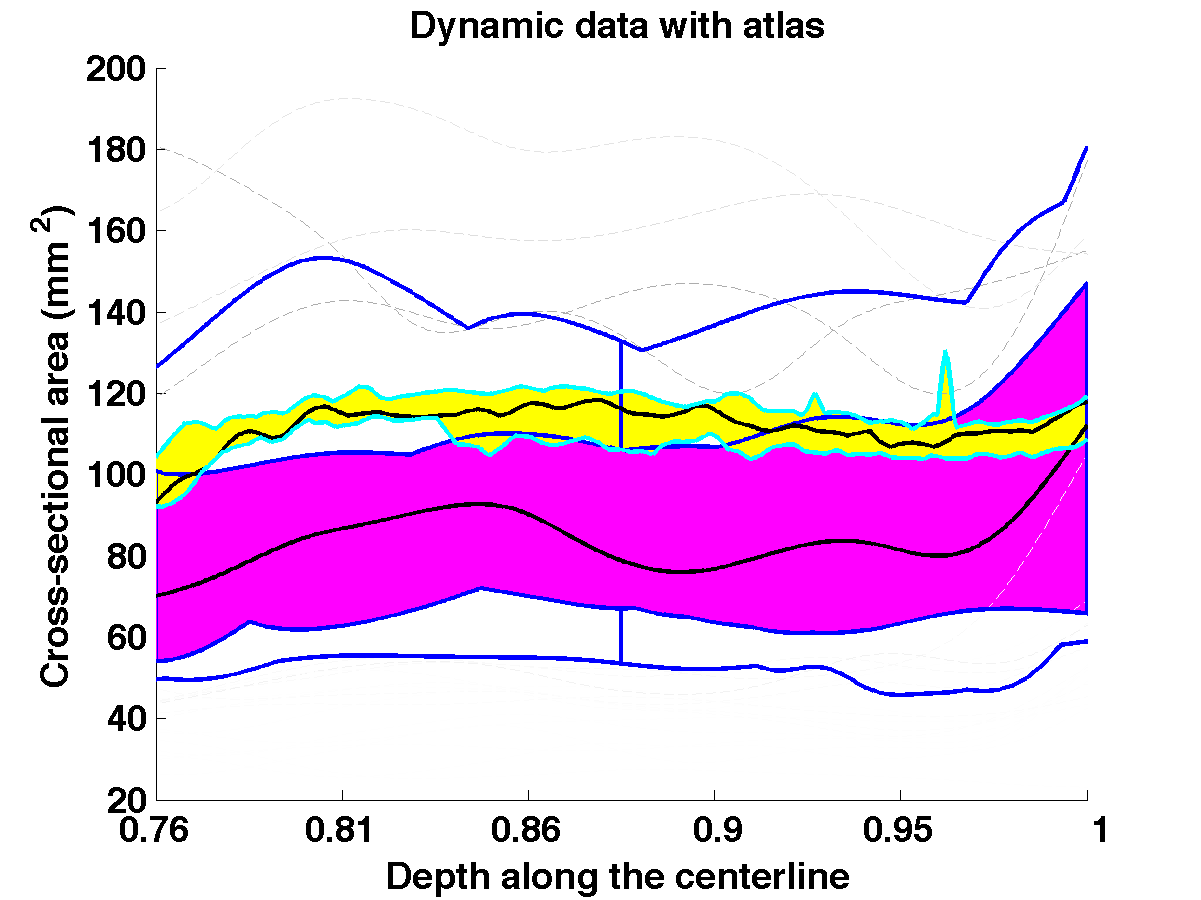
\includegraphics[height=35mm] {fig/Fleck_007_wfbplot.png}
    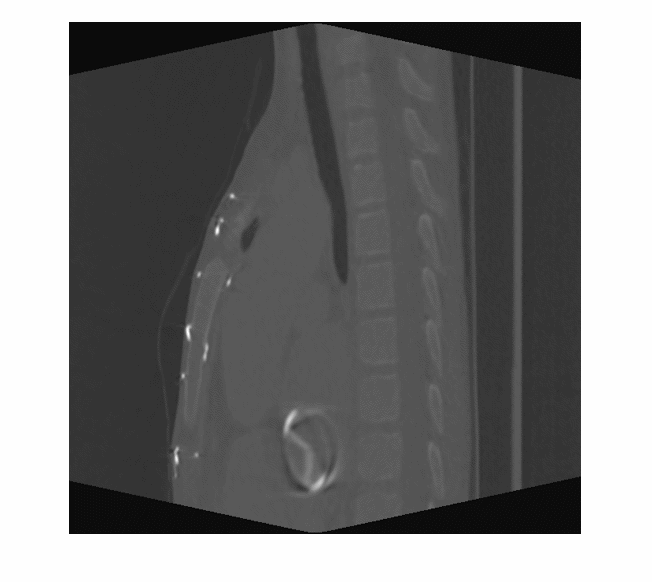
\includegraphics[height=35mm] {fig/Fleck_007.png} \\
    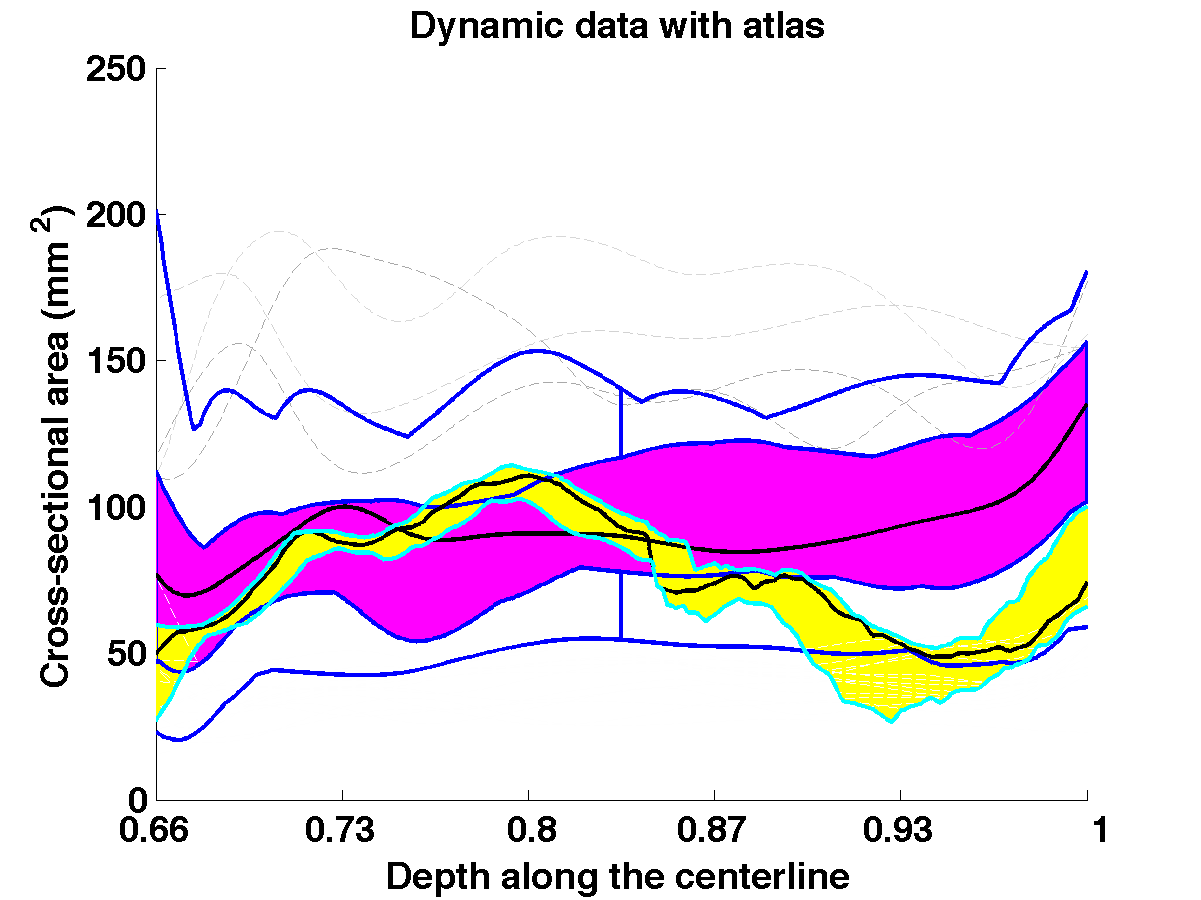
\includegraphics[height=35mm] {fig/Fleck_008_wfbplot.png}
    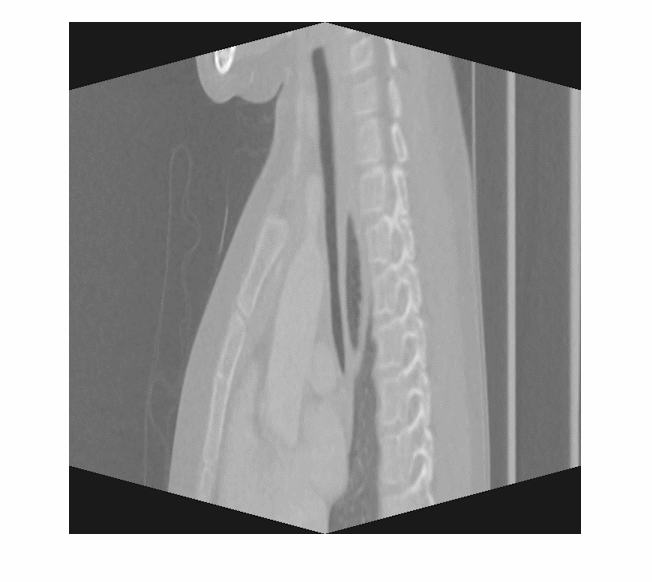
\includegraphics[height=35mm] {fig/Fleck_008.png} \\
    \end{tabular}
    \caption{ \label{fig:Fleck} Dynamic airway atlas for subject Fleck-007 and Fleck-008. The purple area is the interquartile range of normal control atlas. The blue curves are the boundary of the normal control atlas. The yellow area is the entire estimation range of the dynamic subject in different time steps. The depth is in a unified scale, where 0.66 is TVC and 1 is TC.
    }
  \end{center}
\end{figure}